\documentclass[a4paper, 11pt, draft]{report}

\usepackage[utf8]{inputenc} % Texte en utf-8
\usepackage{aeguill}
\usepackage[francais]{babel} % Typographie française
\usepackage[pdftex, hypertexnames=false, colorlinks=true, final]{hyperref}
\usepackage[final]{graphicx}
\usepackage{url} % Gestion des URLs
\usepackage{geometry}
\usepackage{fancyhdr}
\usepackage[Lenny]{fncychap}

% Marges à gauche et à droite de 3cm
\geometry{margin=3cm}

% Utilisation des headers et footers personnalisés de fancyhdr
\pagestyle{fancy}

% Images dans le dossier ./images/
\graphicspath{{./images/}}

% Gestion des métadonnées étranges à rendre visibles au rendu
\newcommand\docname{DINv1.3}
\newcommand\docauthor{Guillaume Bouchard}
\newcommand\docstatus{LIVRABLE} % EN COURS, ATTENTE, VALIDE ou LIVRABLE

% Numérotation mieux ; pour l'instant, on garde le défaut
% \renewcommand\thechapter{\Alph{chapter}}
% \renewcommand\thesection{\Roman{section}}
% \renewcommand\thesubsection{\arabic{subsection}}
% \renewcommand\thesubsubsection{\alph{subsubsection}}

% Format de citation de références standard, marche avec quasiment tout
\newcommand\fullref[1]{\ref{#1}, page \pageref{#1}}

% En-têtes et pieds de page
\lhead{\docname}
\rhead{}
\lfoot{Auteur : H4213}
\cfoot{}
\rfoot{\thepage}

% Titre du document maître
\title{\textbf{COPEVUE}\\
\rule{\textwidth}{1pt}{}\\
\Huge{\textsc{Dossier d'initialisation}}}
\author{\docauthor{}}
\date{\docname{} --- \today{} (\docstatus{})}



\usepackage{rotating}
\newcommand{\ssdsi}{Système de surveillance à distance de sites isolés}
\begin{document}

\maketitle

\tableofcontents

\pagebreak

\chapter{Présentation du projet}

\section{Introduction}

Ce document est le support du chef de projet lors de l'organisation du projet \ssdsi.

\section{Contexte du document}

Ce document se situe en amont de la validation de l'appel d'offres et servira à donner la direction aux études qui seront faites en préalable de l'appel d'offres dans le but de remporter celui-ci.

\section{Documents de références}

Le document à l'origine de ce projet est l'appel d'offres \ssdsi fourni à l'origine par la \emph{COPEVUE}.

L'ensemble des terminologies et abréviations de ce document sont explicités dans le document annexe de l'appel d'offres.

De plus, pour la réalisation de ce projet, les équipes pourront se référer aux documents \emph{Manuel du CdC/RQ,GEI} donnant des directives générales et des conseils pour la bonne marche du projet.

\section{Rappel du problème}
    \subsection{Le contexte}

    La COPEVUE nécessite un système efficace pour effectuer du monitoring distant de ces sites répartis dans le monde dans des sites bien souvent aux conditions climatiques difficiles.

    \subsection{Les objectifs}

    Dans le but de remporter l'appel d'offres, notre équipe doit proposer une solution satisfaisant aux exigences du client, aussi bien au niveau des exigences fonctionnelles que non fonctionnelles.

    Cette étude préalable se doit d'atteindre la qualité nécessaire sans perdre de vue que l'appel d'offres peut ne pas être remporté. De plus elle doit, dans la mesure du possible proposer une solution générique facilement adaptable à tous problèmes d'ordre similaire, dans le but d'être réutilisable.

\section{Les contraintes générales}
% Repompage de faisabilité.tex
    \subsection{Consultation des données} %%%%%
        Les opérateurs ont besoin de pouvoir accéder à tout moment au dernières valeurs transmises par les différents capteurs distants avec la garantie que ces données ne sont pas périmées.

    \subsection{Détection des anomalies} %%%%%
        Toute valeur ou variation anormale d'un capteur distant doit déclencher immédiatement une alarme et le plus souvent possible une réaction automatique du système.

    \subsection{Planification} %%%%%
         Un planning des opérations sur sites -- plein, purge, bilan de routine --
doit être établi afin de minimiser les coûts liés aux transports.

    \subsection{Autonomie} %%%%%
        Les sites distants ont besoin d'être autonomes au maximum pour limiter les déplacements d'agents d'entretien. Il faut donc qu'ils soient capables de recharger leurs batteries, recycler leurs déchets et reconstituer leurs réserves par leur propres moyens.

    \subsection{Fiabilité} %%%%%
        Les systèmes installés sur les sites distants doivent pouvoir fonctionner dans des conditions extrêmes sans se dégrader. Au cas où les conditions empêcheraient le fonctionnement des systèmes, ils doivent se rallumer automatiquement dès que possible.

    \subsection{Maintenance} %%%%%
        Toutes les informations nécessaires à la planification des opérations de maintenance doivent être disponibles dans l'application. De plus, le maximum d'opérations peut être réalisé à distance sans nécessiter le déplacement d'un agent.

    \subsection{Traçabilité} %%%%%
        Toutes les données enregistrées par le système en fonctionnement ainsi que les actions des intervenants doivent être enregistrées afin de traiter \emph{a posteriori} des cas d'erreur ou de procéder à une analyse des données dans un but statistique.

    \subsection{Ergonomie} %%%%%
        Les interfaces doivent rester simples et facilement utilisables par des utilisateurs peu familiarisés avec l'informatique.

\chapter{Tâches et acteurs}

% fin du repompage
\section{Organisation du travail}
    \subsection{Chef de projet et coordinateur}
        \paragraph{Guillaume Bouchard} anime l'équipe et les séances de travail. Il a une vue d'ensemble du projet et de ses objectifs et il planifie le déroulement de l'étude.

    \subsection{Responsable qualité}
        \paragraph{Fabrice Gabolde} épaule le chef de projet dans son travail en définissant l'environnent de qualité dans lequel le projet doit se dérouler.
        
    \subsection{GEI}
        Cette équipe est composée de 4 personnes qui représentent les experts sur ce projet. Il sont chargés de l'étude technique du projet : 
        \begin{itemize}
            \item Guillaume Ayoub
            \item Pierre-Yves David
            \item Remi Thévenoux
            \item Nicolas Kandel
       \end{itemize}

\section{Liste des livrables attendus}

Cette section décrit de façon simple les livrables attendus. Ceux dont le nom est suivi d'un astérisque n'existent que de façon interne et ne seront pas livrés au client.
    \subsection{CdC}
        \paragraph{Fiche d'argumentation commerciale} Il s'agit d'une plaquette de deux pages présentant les avantages de notre réalisation. Elle doit s'effectuer dans une optique très commerciale.
        \paragraph{Procédure de réalisation d'un dossier d'initialisation*} Il s'agit d'un dossier visant à guider tout chef de projet dans la réalisation du dossier d'initialisation.
        \paragraph{Dossier d'initialisation*} Il s'agit de ce dossier même.
        \paragraph{Dossier Bilan*} Ce dossier d'un maximum de 5 pages est un bilan du point du vu du management en tant que chef de projet.
        \paragraph{PMP*} Ce document a pour but de décrire le pilotage de tout le projet (et pas seulement la partie visant à remporter l'appel d'offres).
    \subsection{RQ}
        \paragraph{Gestion de la documentation*} L'objectif de ce dossier est de définir des règles communes pour les livrables et la documentation.
        \paragraph{Dossier de synthèse} Ce document fera la synthèse du projet et du travail du GEI.
        \paragraph{Fiches d'aide à la rédaction de procédures et CdC logiciels*} Il s'agit de bonnes pratiques et de plans types pour la réalisation de ce type de document.
        \paragraph{PAQP*} Plan d'assurance qualité projet simplifié.
        \paragraph{PAQL*} Ébauche de PAQL.
        \paragraph{Bilan critique*} Ce document est une critique des différents livrables fournis par les autres équipes.
    \subsection{GEI}
        \paragraph{Dossier de faisabilité} Il évoque les différentes problématiques techniques qui vont se poser lors de la réalisation de ce projet et propose des grandes lignes de solution. Ce document est là pour prouver que ce bureau d'étude peut réaliser le projet.
        \paragraph{Dossier de spécification technique des besoins} Il traduit les besoins fonctionnels et non fonctionnels en contraintes techniques.
        \paragraph{Dossier de conception} Ce dossier présente la conception du système dans sa globalité dans le but de montrer que ce bureau d'étude sait comment réaliser le produit. Cependant il reste de très haut niveau et ne rentrera pas dans les détails.
        \paragraph{Dossier des interfaces de communications} Ce dossier exprime les besoins en interfaces des différents sous projets pour permettre à chacun d'appréhender les projets avec lesquels il devra communiquer.
        \paragraph{Cahiers des charges} Dans le but de réaliser le projet dans la globalité, auront été isolés différents sous projets qui nécessitent un cahier des charges (dans le but de sous-traiter par exemple). 
        Les trois cahiers des charges à réaliser correspondront à :
        \begin{itemize}
            \item Système distant ;
            \item Système central ;
            \item Système de l'intervenant.
        \end{itemize}

        Ce choix vient du fait que ces trois sous-ensembles sont les plus importants du projets (si on exclut les sous-ensembles non fonctionnels ou transversaux) et qu'il ne couvrent en grande partie que du logiciel, ce qui semble plus simple à appréhender.

    \subsection{Bilan personnel}
        Ce bilan, d'une page maximum et demandé à tous les collaborateurs, est là pour permettre à l'élève de réflechir a son expérience au sein du projet ingénierie 4IF.

\chapter{Organisation du projet}

\section{Organisation par groupes}

Dans ce projet, on a distingué trois groupes de collaborateurs : le chef de projet, le responsable qualité et le groupe d'étude. Le fonctionnement de chaque groupe étant totalement diffèrent, leur organisation s'en ressent.

    \subsection{Chef de projet}

Celui-ci est autonome et le seul document qu'il doit réaliser qui ait un impact sur le travail des autres est son dossier d'initialisation, réalisé en début de projet. Pour tout ses autres documents, celui-ci organisera son travail comme il le désire en gardant en tête que ceux-ci sont à faire viser par le RQ, il devra donc se mettre d'accord avec lui sur la date de rendu.

    \subsection{Responsable qualité}

        Il doit fournir son dossier de documentation le plus rapidement possible en début de projet (de la même manière que le chef de projet fournit son dossier d'initialisation). Tout ses autres documents n'ont pas d'application sur le travail des autres membres de l'équipe, il peut donc organiser son temps comme il le désire à condition de respecter la deadline de fin.

        Cependant il peut préparer son organisation en fonction des deadlines du groupe d'étude, puisque il doit valider et analyser tous les documents fournis par celui-ci.

    \subsection{Groupe d'étude}

    Il s'agit du seul groupe qui a un travail collaboratif et en parallèle, c'est pourquoi celui-ci nécessite une organisation précise et minutieuse qui sera décrite dans la suite de ce document.


\section{Organigramme des tâches}
    \subsection{Macro-phasage}
        On distinguera deux phases dans le projet :
        \paragraph{La phase d'initialisation} Dans celle-ci, le CdC et le RQ mettent en place les fondements de l'étude (organisation, politique de qualité) tandis que les GEI dégrossissent l'étude préalable avec les drafts des livrables.
        \paragraph{La phase de finalisation} Après avoir présenté et validé avec le client l'orientation prise par l'étude, les documents finaux seront rendus après modification des derniers points de détails. Le CdC aura à sa charge de préparer la présentation du produit au client.
    \subsection{Gantt}
    La planification de la répartition du travail est fournie avec les diagrammes de Gantt suivants.

    Il faut bien prendre en compte que ces diagrammes indiquent la répartition du travail par personne ainsi que l'ordonnancement des tâches, mais ils ne sont en aucun cas contractuels en ce qui concerne le temps imparti ainsi que la plage horaire utilisée, un membre d'une équipe n'a pas de contraintes sur sa manière d'organiser son temps, à la condition qu'il fournisse ses travaux suivant le planning.
    Le travail du chef de projet est de s'assurer que ce planning est bien suivi.

    On distingue tout de même deux parties, correspondant respectivement aux semaines 1 à 3 et 4 à 5.

	\begin{sidewaysfigure}[htbp]
	\begin{center}
	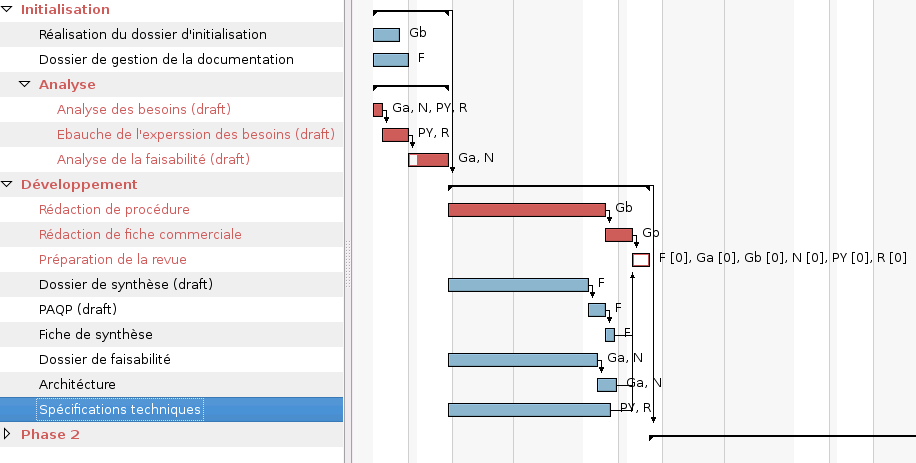
\includegraphics[width=\textwidth]{gantt1.png}
    \caption{Organisation de la première partie}
	\end{center}
	\end{sidewaysfigure}
	
    \begin{sidewaysfigure}[htbp]
	\begin{center}
	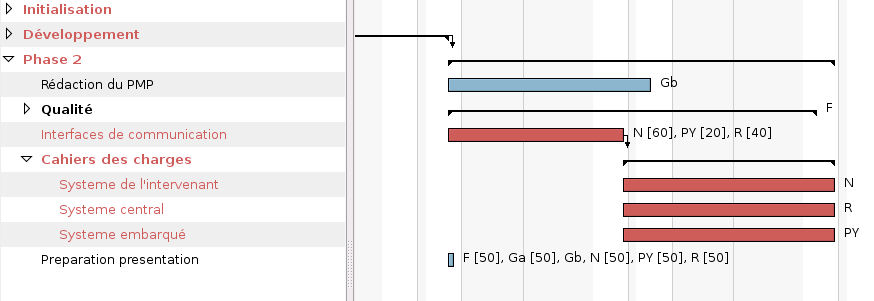
\includegraphics[width=\textwidth]{gantt2.png}
    \caption{Organisation de la seconde partie}
	\end{center}
	\end{sidewaysfigure}

\section{Modalités de suivi}
    \subsection{Les règles de suivi}
    Lors d'un bilan en fin de séance, on effectuera la vérification de la conformité de l'avancement avec le planning prévu.

    Dans le cas de non conformité, on essayera de savoir pourquoi. Dans le cas d'un problème d'organisation de l'équipe responsable, on tentera d'y remédier. Tout autre problème (quantité de travail mal évaluée, difficulté technique) peut être contourné plus simplement en s'octroyant du temps supplémentaire affecté à la tâche en question.

    \subsection{Les outils utilisés}

Diagramme de Gantt, suivi de projet. Utilisation de subversion pour le travail collaboratif sur les rapports.

\section{Gestion des risques}
    \subsection{Risques concernant l'application du projet}

    Le sujet ne mettant pas en jeu des risques techniques excessifs, on ne prendra pas de mesures particulières pour limiter les risques.

    \subsection{Risques propres au projet}

    Le risque principal est le non remport de l'appel d'offres. L'approche du projet en tant que développement pouvant être générique permet de réduire les risques de perte financières dans ce cas.

    On peut aussi remarquer les risques de non respect des deadlines pour certains collaborateurs -- quelle que soit la raison, mauvaise volonté, maladie\ldots Ce risque est inévitable, mais le chef de projet peut, avec une bonne communication, pouvoir prévoir et ainsi gérer ceux-ci du mieux possible.

\end{document}

